%-------------------------------------------------------------------------------
\usetikzlibrary{calc}
%coordinate test point. Use as follows: 	\coordinate (cen) 	 	 at (0,0) (cen) [point];
\tikzset{
	every point/.style = {radius={\pgflinewidth}, opacity=1, draw, solid, fill=white},
	pt/.pic = {
		\begin{pgfonlayer}{foreground}
			\path[every point, #1] circle;
		\end{pgfonlayer}
	},
	point/.style={insert path={pic{pt={#1}}}}, point/.default={},
	point name/.style = {insert path={coordinate (#1)}}
}
%-------------------------------------------------------------------------------

% basic delacations
\pgfdeclarelayer{background}%
\pgfdeclarelayer{foreground}%
\pgfsetlayers{background,main,foreground}%

%Coin Symbol--------------------------------------------------------------------
\tikzset{%
	pics/coin/.style n args={3}{%
		code ={
			\def \coinLineWidth {#1}%
			\def \coinCenDist   {#2}%
			\def \circRad       {#3}%
			\def \signRad       {\circRad*0.20}%
			\def \signRadProp   {0.45}
			\def \signRadExt    {\signRad*\signRadProp}
			\def \signRadOut    {\signRad+\signRadExt}
			\def \signAngle     {30}
			\def \sinSignAngle  {sin(\signAngle)}
			\def \cosSignAngle  {cos(\signAngle)}
			\def \signWidth     {{pow((pow(\signRadOut,2)-pow(\sinSignAngle*\signRad,2)),0.5)-(\cosSignAngle)*\signRad)}}
			
			\def \startIX       {{cos(\signAngle)*\signRad}}
			\def \startIY       {{\sinSignAngle*\signRad}}
			
			\def \startOY       {\startIY}
			\def \signAngleOutS {{atan((\sinSignAngle*\signRad)/pow((pow(\signRadOut,2)-pow(\sinSignAngle*\signRad,2)),0.5))}}
			\def \signAngleOutE {{360-atan((\sinSignAngle*\signRad)/pow((pow(\signRadOut,2)-pow(\sinSignAngle*\signRad,2)),0.5))}}
	%
			\coordinate ()          at ( 0.0     , 0.0);%
			\coordinate (cen)       at ( 0.0     , 0.0);%
			\coordinate (cenB)      at ($(cen)    + ( 0.00,-\coinCenDist)$);%
						
			\node[
				circle,
				draw = black,
				fill = white,
				line width = \coinLineWidth,
				minimum size = \circRad,
				inner sep = 0pt,
				outer sep = 0pt,
			](NCD) at (cenB) {};
			
			\node[
				circle,
				draw = black,
				fill = white,
				line width = \coinLineWidth,
				minimum size = \circRad,
				inner sep = 0pt,
				outer sep = 0pt,
			](NCU) at (cen) {};
			
%			\draw[ - , line width = \coinLineWidth, black] (NCU.195) -- (NCD.195);
			\draw[-, line width = \coinLineWidth, black] (NCU.210) -- (NCD.210);
			\draw[-, line width = \coinLineWidth, black] (NCU.225) -- (NCD.225);
			\draw[-, line width = \coinLineWidth, black] (NCU.240) -- (NCD.240);
			\draw[-, line width = \coinLineWidth, black] (NCU.255) -- (NCD.255);
			\draw[-, line width = \coinLineWidth, black] (NCU.270) -- (NCD.270);
			\draw[-, line width = \coinLineWidth, black] (NCU.285) -- (NCD.285);
			\draw[-, line width = \coinLineWidth, black] (NCU.300) -- (NCD.300);
			\draw[-, line width = \coinLineWidth, black] (NCU.315) -- (NCD.315);
			\draw[-, line width = \coinLineWidth, black] (NCU.330) -- (NCD.330);
%			\draw[ - , line width = \coinLineWidth, black] (NCU.345) -- (NCD.345);
			
			\draw[
				 - ,
				 line width = \coinLineWidth,
				 black!80!white,
				 fill = black!80!white
			]
				(\startIX,-\startIY) arc (360-\signAngle:\signAngle:\signRad)
				-- +(\signWidth, 0.0)
				arc (\signAngleOutS:\signAngleOutE:\signRadOut)
				-- (\startIX,-\startIY)
				-- cycle
				;
		}%
		
	} ,%
	pics/coin/.default={1.0pt}{0.1}{1cm}%
}%
%
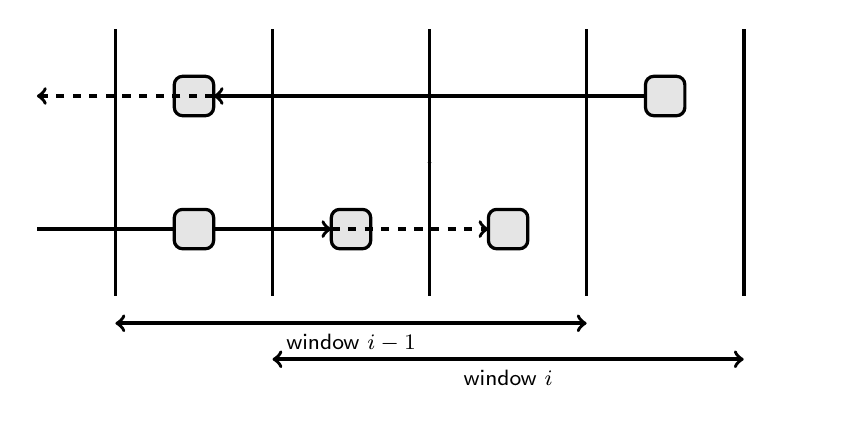
\begin{tikzpicture}
	\def \debugPoint   {}%
%	\def \debugPoint   {point}%
	\def \debugPointF  {point}%
	% font settings ############################################################
	\def \fontset      {\scriptsize\sffamily}
	\def \fontsetB     {\footnotesize\sffamily}
	% color definition #########################################################
	\def \colorOut     {black!100!white}
	\def \colorIn      {black!10!white}
	% arrow and line definitions ###############################################
	\def \lineW        {1.3pt}
	% width/height definition ##################################################
	\def \picW         {\columnwidth*25.5/31}%
	\def \picH         {\paperheight*3.75/31}%
	\def \TH           {\picH*0.4}%picH*0.5*0.8

	\def \DayD         {\picW*1/10}
	\def \BorD         {1em}

	% tikz styles################################################################
	\tikzstyle{lineIO} = [
		- ,
		line width = \lineW*0.8,
	]
	\tikzstyle{nodeOuter}   = [
		draw,
		rectangle,
		rounded corners=5pt,
		solid,
		line width = \lineW,
		black,
		inner sep = 0pt,
		outer sep = 0pt,
		text width = \BOW,
		minimum width = \BOW,
		minimum height = \BOH*1.075,
	]
	\tikzstyle{nodeInner}   = [
		draw,
		rectangle,
		rounded corners=3pt,
		solid,
		line width = \lineW*0.9,
		black,
		fill = \colorIn,
		inner sep = 0pt,
		outer sep = 0pt,
		align = center,
		text width = 0.5cm,
		minimum width = 0.5cm,
		minimum height = 0.5cm,
	]
	% coordinates ###############################################################
	% 1 | 2 | 3 | 4 | 5 | 6 | 7 | 8 | 9 | 10 | 11 | 12 | 13 | 14 |
	% A | B | C | D | E | F | G | H | I |  J |  K |  L |  M |  N |

	\coordinate (cen)       at ($(0.0,0.0)   + ( 0.0       , 0.0         )$) (cen)   [\debugPoint];%

	\coordinate (PLU)       at ($(cen)       + (-\picW*0.5 , \picH*0.5   )$) (PLU)   [\debugPoint];%
	\coordinate (PLD)       at ($(cen)       + (-\picW*0.5 ,-\picH*0.5   )$) (PLD)   [\debugPoint];%
	\coordinate (PRU)       at ($(cen)       + ( \picW*0.5 , \picH*0.5   )$) (PRU)   [\debugPoint];%
	\coordinate (PRD)       at ($(cen)       + ( \picW*0.5 ,-\picH*0.5   )$) (PRD)   [\debugPoint];%

	\coordinate (BCU)       at ($(cen)       + ( \picW*0.0 , \picH*0.5   )$) (BCU)   [\debugPoint];%
	\coordinate (BCD)       at ($(cen)       + ( \picW*0.0 ,-\picH*0.5   )$) (BCD)   [\debugPoint];%

	\coordinate (BLAU)      at ($(cen)       + (-\DayD*1.0 , \picH*0.5   )$) (BLAU)  [\debugPoint];%
	\coordinate (BLAD)      at ($(cen)       + (-\DayD*1.0 ,-\picH*0.5   )$) (BLAD)  [\debugPoint];%
	\coordinate (BLADD)     at ($(BLAD)      + ( 0.0       ,-\BorD*1.0   )$) (BLADD) [\debugPoint];%
	\coordinate (BLBU)      at ($(cen)       + (-\DayD*2.0 , \picH*0.5   )$) (BLBU)  [\debugPoint];%
	\coordinate (BLBD)      at ($(cen)       + (-\DayD*2.0 ,-\picH*0.5   )$) (BLBD)  [\debugPoint];%
	\coordinate (BLBDD)     at ($(BLBD)      + ( 0.0       ,-\BorD*1.0   )$) (BLBDD) [\debugPoint];%
	\coordinate (BLCU)      at ($(cen)       + (-\DayD*3.0 , \picH*0.5   )$) (BLCU)  [\debugPoint];%
	\coordinate (BLCD)      at ($(cen)       + (-\DayD*3.0 ,-\picH*0.5   )$) (BLCD)  [\debugPoint];%
	\coordinate (BLCDD)     at ($(BLCD)      + ( 0.0       ,-\BorD*1.0   )$) (BLCDD) [\debugPoint];%
	\coordinate (BLDU)      at ($(cen)       + (-\DayD*4.0 , \picH*0.5   )$) (BLDU)  [\debugPoint];%
	\coordinate (BLDD)      at ($(cen)       + (-\DayD*4.0 ,-\picH*0.5   )$) (BLDD)  [\debugPoint];%
	\coordinate (BLDDD)     at ($(BLDD)      + ( 0.0       ,-\BorD*1.0   )$) (BLDDD) [\debugPoint];%
%	\coordinate (BLEU)      at ($(cen)       + (-\DayD*4.5 , \picH*0.5   )$) (BLEU)  [\debugPoint];%
%	\coordinate (BLED)      at ($(cen)       + (-\DayD*4.5 ,-\picH*0.5   )$) (BLED)  [\debugPoint];%

	\coordinate (BRAU)      at ($(cen)       + ( \DayD*1.0 , \picH*0.5   )$) (BRAU)  [\debugPoint];%
	\coordinate (BRAD)      at ($(cen)       + ( \DayD*1.0 ,-\picH*0.5   )$) (BRAD)  [\debugPoint];%
	\coordinate (BRADD)     at ($(BRAD)      + ( 0.0       ,-\BorD*1.0   )$) (BRADD) [\debugPoint];%
	\coordinate (BRBU)      at ($(cen)       + ( \DayD*2.0 , \picH*0.5   )$) (BRBU)  [\debugPoint];%
	\coordinate (BRBD)      at ($(cen)       + ( \DayD*2.0 ,-\picH*0.5   )$) (BRBD)  [\debugPoint];%
	\coordinate (BRBDD)     at ($(BRBD)      + ( 0.0       ,-\BorD*1.0   )$) (BRBDD) [\debugPoint];%
	\coordinate (BRCU)      at ($(cen)       + ( \DayD*3.0 , \picH*0.5   )$) (BRCU)  [\debugPoint];%
	\coordinate (BRCD)      at ($(cen)       + ( \DayD*3.0 ,-\picH*0.5   )$) (BRCD)  [\debugPoint];%
	\coordinate (BRCDD)     at ($(BRCD)      + ( 0.0       ,-\BorD*1.0   )$) (BRCDD) [\debugPoint];%
	\coordinate (BRDU)      at ($(cen)       + ( \DayD*4.0 , \picH*0.5   )$) (BRDU)  [\debugPoint];%
	\coordinate (BRDD)      at ($(cen)       + ( \DayD*4.0 ,-\picH*0.5   )$) (BRDD)  [\debugPoint];%
	\coordinate (BRDDD)     at ($(BRDD)      + ( 0.0       ,-\BorD*1.0   )$) (BRDDD) [\debugPoint];%
%	\coordinate (BLDU)      at ($(cen)       + ( \DayD*4.5 , \picH*0.5   )$) (BLDU)  [\debugPoint];%
%	\coordinate (BLDD)      at ($(cen)       + ( \DayD*4.5 ,-\picH*0.5   )$) (BLDD)  [\debugPoint];%

	%clipping
%	\clip ($(PLD) + ( 0.0 ,-0.5)$) rectangle ($(PRU) + ( 0.0 , 0.1)$);
	%basic picture

	\draw[<->, solid, line width =\lineW] (BLDDD) -- node [midway, below] {\fontsetB{}window $i-1$} (BRBDD);
	\draw[<->, solid, line width =\lineW] ($(BLBDD) + ( 0.0,-\BorD*1.3)$) -- node [midway, below] {\fontsetB{}window $i$} ($(BRDDD) + ( 0.0,-\BorD*1.3)$);

	\draw[ -, solid , line width = \lineW] (BCU)   -- (BCD);
	\draw[ -, solid , line width = \lineW] (BLBU)  -- (BLBD);
	\draw[ -, solid , line width = \lineW] (BLDU)  -- (BLDD);
	\draw[ -, solid , line width = \lineW] (BRBU)  -- (BRBD);
	\draw[ -, solid , line width = \lineW] (BRDU)  -- (BRDD);

	%Nodes
	\node[nodeInner] (NRCA) at ($(BRCU)!0.25!(BRCD)$) {};
	\node[nodeInner] (NLCA) at ($(BLCU)!0.25!(BLCD)$) {};
	\node[point]     (NLEA) at ($(PLU)!0.25!(PLD)$) {};


	\node[nodeInner] (NLCB) at ($(BLCU)!0.75!(BLCD)$) {};
	\node[]          (NLEB) at ($(PLU)!0.75!(PLD)$) {};
	\node[nodeInner] (NLAB) at ($(BLAU)!0.75!(BLAD)$) {};
	\node[nodeInner] (NRAB) at ($(BRAU)!0.75!(BRAD)$) {};

	%Arrows depending on nodes
	\draw[ ->, line width = \lineW] (NRCA.west) -- (NLCA.east);
	\draw[ ->, line width = \lineW, dashed] (NLCA.east) -- (NLEA.center);

	\draw[ - , line width = \lineW] (NLCB.west) -- (NLEB.center);
	\draw[ ->, line width = \lineW] (NLCB.east) -- (NLAB.west);
	\draw[ ->, line width = \lineW, dashed] (NLAB.west) -- (NRAB.west);
\end{tikzpicture} 